\documentclass[11pt,letterpaper]{article}

% --- Fonts and encoding ---
\usepackage[T1]{fontenc}
\usepackage{mathpazo}
\usepackage{microtype}

% --- Page geometry ---
\usepackage[margin=0.95in]{geometry}

% --- Graphics and diagrams ---
\usepackage{tikz}
\usetikzlibrary{arrows.meta,positioning,calc,fit,shapes.geometric,backgrounds,decorations.pathmorphing}

% --- Colors ---
\definecolor{accent}{HTML}{2E4057}
\definecolor{midgray}{HTML}{6B7280}
\definecolor{muted}{HTML}{8B8B8B}
\definecolor{deepred}{HTML}{9B2335}
\definecolor{deepblue}{HTML}{1E3A5F}
\definecolor{teal}{HTML}{0D7377}
\definecolor{amber}{HTML}{B8860B}
\definecolor{softblue}{HTML}{D6E4F0}
\definecolor{softred}{HTML}{F0D6D6}
\definecolor{softgreen}{HTML}{D6F0D6}
\definecolor{softyellow}{HTML}{F5F0D0}
\definecolor{softpurple}{HTML}{E4D6F0}
\definecolor{nodebg}{HTML}{EEF1F6}
\definecolor{portalbg}{HTML}{E0F0E0}
\definecolor{dialecticbg}{HTML}{F0E0E8}

% --- Section formatting ---
\usepackage{titlesec}
\titleformat{\section}{\large\bfseries\color{accent}}{\thesection}{1em}{}
\titleformat{\subsection}{\normalsize\bfseries\color{accent}}{\thesubsection}{1em}{}
\titleformat{\subsubsection}{\small\bfseries\color{deepblue}}{\thesubsubsection}{1em}{}

% --- Headers/footers ---
\usepackage{fancyhdr}
\pagestyle{fancy}
\fancyhf{}
\fancyhead[L]{\footnotesize\textsc{\color{midgray}Theseus}}
\fancyhead[R]{\footnotesize\textsc{\color{midgray}Noosphere Project Status}}
\fancyfoot[C]{\footnotesize\thepage}
\renewcommand{\headrulewidth}{0.4pt}

% --- Tables ---
\usepackage{booktabs}
\usepackage{tabularx}
\usepackage{array}

% --- Hyperlinks ---
\usepackage[colorlinks=true,linkcolor=accent,citecolor=accent,urlcolor=teal]{hyperref}

% --- Math ---
\usepackage{amsmath,amssymb}

\setlength{\parskip}{4pt plus 1pt minus 1pt}
\setlength{\parindent}{0pt}

% ====================================================================
\begin{document}

\thispagestyle{empty}

\vspace*{1cm}

\begin{center}
{\Large\bfseries\color{accent} Noosphere: The Communal Brain of the Firm}\\[8pt]
{\large\color{midgray} Project Status and Architectural Overview}\\[16pt]
{\normalsize Theseus Research Division}\\[4pt]
{\footnotesize\color{muted} April 2026}
\end{center}

\vspace{0.5cm}
\hrule
\vspace{0.3cm}
\tableofcontents
\vspace{0.3cm}
\hrule

\newpage

% ====================================================================
\section{Executive Summary}

Noosphere is a computational epistemology system: a software engine that ingests the intellectual output of Theseus's founders---podcast transcripts, essays, annotations, discussions---and distils it into a structured, queryable, evolving knowledge graph. Its purpose is not to store information but to \emph{reason about reasoning}: to detect contradictions, track conviction drift, classify discourse types, attribute ideas to founders, and measure the coherence of the firm's collective thought.

The system now comprises three major subsystems:

\begin{enumerate}
\item \textbf{Noosphere Core} --- A 15-module Python backend implementing a 6-layer coherence engine, embedding geometry analysis, temporal tracking, discourse classification, and automated post-discussion synthesis. Approximately 5,500 lines of Python.

\item \textbf{Founder Portal} --- A Next.js 16 web application that provides founders with authenticated access to upload content, trigger ingestion, and view the state of the knowledge graph. Built on React 19, Prisma 7, and SQLite.

\item \textbf{Dialectic} --- A live conversation analysis application (new, v0.1) that records audio, transcribes in real time, and provides a dashboard of live epistemological feedback: contradiction detection, topic tracking, open-loop identification, and question generation.
\end{enumerate}

% ====================================================================
\section{System Architecture}

\begin{center}
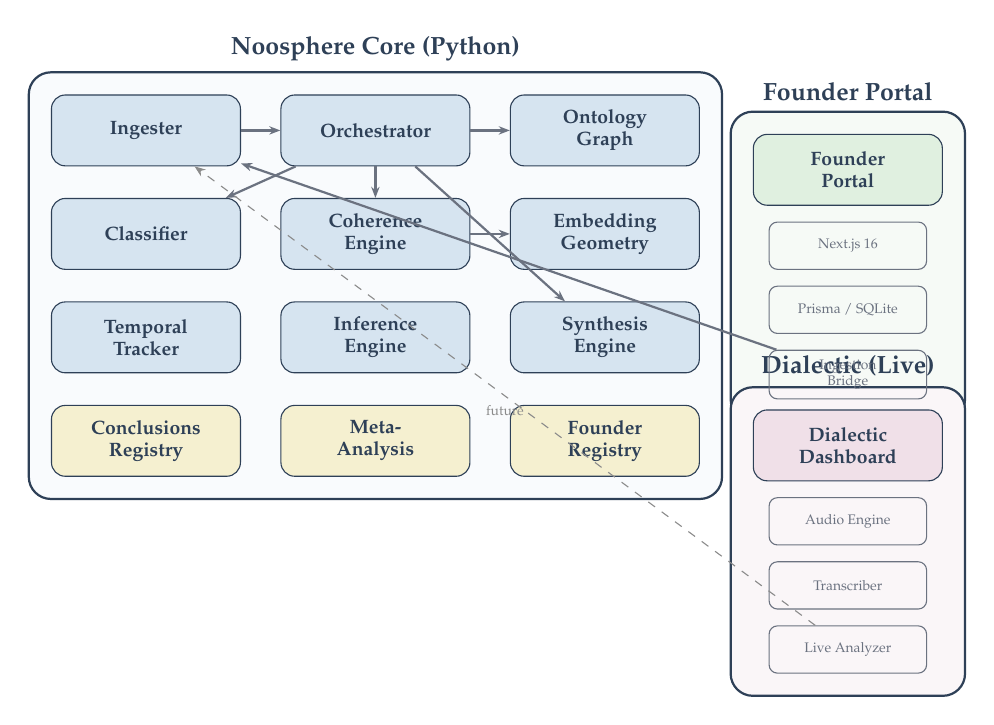
\begin{tikzpicture}[
    node distance=0.6cm and 0.8cm,
    block/.style={draw=accent, rounded corners=5pt, minimum width=2.4cm, minimum height=0.9cm, align=center, font=\scriptsize\bfseries, text=accent},
    smallblock/.style={draw=midgray, rounded corners=3pt, minimum width=2cm, minimum height=0.6cm, align=center, font=\tiny, text=midgray},
    bigbox/.style={draw=accent, rounded corners=8pt, thick, inner sep=8pt},
    arrow/.style={-{Stealth[length=4pt]}, thick, color=midgray},
    dasharrow/.style={-{Stealth[length=4pt]}, dashed, color=muted},
]

% --- Noosphere Core ---
\node[block, fill=softblue] (orch) at (0,0) {Orchestrator};
\node[block, fill=softblue, left=0.5cm of orch] (ing) {Ingester};
\node[block, fill=softblue, right=0.5cm of orch] (onto) {Ontology\\Graph};

\node[block, fill=softblue, below=0.4cm of ing] (class) {Classifier};
\node[block, fill=softblue, below=0.4cm of orch] (coh) {Coherence\\Engine};
\node[block, fill=softblue, below=0.4cm of onto] (geom) {Embedding\\Geometry};

\node[block, fill=softblue, below=0.4cm of class] (temp) {Temporal\\Tracker};
\node[block, fill=softblue, below=0.4cm of coh] (inf) {Inference\\Engine};
\node[block, fill=softblue, below=0.4cm of geom] (synth) {Synthesis\\Engine};

\node[block, fill=softyellow, below=0.4cm of temp] (conc) {Conclusions\\Registry};
\node[block, fill=softyellow, below=0.4cm of inf] (meta) {Meta-\\Analysis};
\node[block, fill=softyellow, below=0.4cm of synth] (found) {Founder\\Registry};

% Bounding box
\begin{scope}[on background layer]
\node[bigbox, fill=softblue!15, fit=(ing)(onto)(conc)(found), label={[font=\small\bfseries,color=accent]above:Noosphere Core (Python)}] {};
\end{scope}

% --- Founder Portal ---
\node[block, fill=portalbg] (portal) at (6, -0.5) {Founder\\Portal};
\node[smallblock, below=0.2cm of portal] (next) {Next.js 16};
\node[smallblock, below=0.2cm of next] (prisma) {Prisma / SQLite};
\node[smallblock, below=0.2cm of prisma] (ingestlib) {Ingestion\\Bridge};

\begin{scope}[on background layer]
\node[bigbox, fill=portalbg!30, fit=(portal)(ingestlib), label={[font=\small\bfseries,color=accent]above:Founder Portal}] {};
\end{scope}

% --- Dialectic ---
\node[block, fill=dialecticbg] (dial) at (6, -4) {Dialectic\\Dashboard};
\node[smallblock, below=0.2cm of dial] (audio) {Audio Engine};
\node[smallblock, below=0.2cm of audio] (trans) {Transcriber};
\node[smallblock, below=0.2cm of trans] (anlz) {Live Analyzer};

\begin{scope}[on background layer]
\node[bigbox, fill=dialecticbg!30, fit=(dial)(anlz), label={[font=\small\bfseries,color=accent]above:Dialectic (Live)}] {};
\end{scope}

% --- Arrows ---
\draw[arrow] (ingestlib) -- (ing);
\draw[arrow] (ing) -- (orch);
\draw[arrow] (orch) -- (onto);
\draw[arrow] (orch) -- (coh);
\draw[arrow] (orch) -- (class);
\draw[arrow] (coh) -- (geom);
\draw[arrow] (orch) -- (synth);
\draw[dasharrow] (anlz) -- node[below, font=\tiny, text=muted] {future} (ing);

\end{tikzpicture}
\end{center}

% ====================================================================
\section{Noosphere Core: Module-by-Module}

The core engine is a Python package (\texttt{noosphere/noosphere/}) comprising fifteen modules. The \textbf{Orchestrator} is the central coordinator; all other modules are lazy-loaded as needed.

\subsection{Data Models (\texttt{models.py}, ${\sim}280$ lines)}

All data structures are Pydantic \texttt{BaseModel}s, ensuring runtime validation and serialisation. The principal types:

\begin{tabularx}{\textwidth}{lX}
\toprule
\textbf{Type} & \textbf{Purpose} \\
\midrule
\texttt{Claim} & Atomic proposition extracted from a transcript or essay. Carries speaker attribution, timestamp, embedding vector, confidence score, and discipline tag. \\
\texttt{Principle} & A distilled, stable belief synthesised from multiple claims. Includes a chain of supporting evidence, founder contribution weights, and conviction level. \\
\texttt{Episode} & Metadata for a podcast episode or discussion session. \\
\texttt{CoherenceReport} & Full 6-layer coherence assessment with identified contradictions and weak links. \\
\texttt{FounderProfile} & Persistent intellectual fingerprint for each founder. \\
\texttt{TemporalSnapshot} & A principle's state at a point in time: conviction, embedding, drift from origin. \\
\texttt{Conclusion} & A substantive claim (separated from methodological principles) with calibration metadata. \\
\bottomrule
\end{tabularx}

The type system enforces a strict separation between \emph{methodological principles} (how to think) and \emph{substantive conclusions} (what to believe), reflecting Theseus's meta-methodological orientation.

\subsection{Orchestrator (\texttt{orchestrator.py}, ${\sim}500$ lines)}

The orchestrator runs a 10-step ingestion pipeline:

\begin{enumerate}
\item \textbf{Parse} --- Transcript or written input is segmented into speaker-attributed chunks.
\item \textbf{Extract Claims} --- An LLM (Claude) identifies atomic propositional claims.
\item \textbf{Embed} --- Each claim is embedded via SBERT (\texttt{all-MiniLM-L6-v2}).
\item \textbf{Classify} --- Each claim is tagged as METHODOLOGICAL, SUBSTANTIVE, META\_METHODOLOGICAL, MIXED, or NON\_PROPOSITIONAL.
\item \textbf{Route} --- Methodological claims enter the ontology graph; substantive claims enter the conclusions registry.
\item \textbf{Distil Principles} --- Claims are clustered and distilled into stable principles via LLM synthesis.
\item \textbf{Coherence Check} --- The 6-layer coherence engine scores the updated graph.
\item \textbf{Temporal Snapshot} --- Principle states are recorded for drift analysis.
\item \textbf{Persist} --- The graph and all metadata are serialised to disk.
\item \textbf{Post-Discussion Synthesis} --- The SynthesisEngine generates five outputs (see \S\ref{sec:synthesis}).
\end{enumerate}

\subsection{Ingester (\texttt{ingester.py}, ${\sim}300$ lines)}

Handles three input formats: timestamped transcripts (e.g., \texttt{[00:01:23] Speaker: text}), labelled transcripts (speaker labels without timestamps), and unstructured text. The claim extractor batches segments and calls Claude with a structured prompt that demands atomic, falsifiable propositions.

\subsection{Ontology Graph (\texttt{ontology.py}, ${\sim}400$ lines)}

A \texttt{networkx} directed graph where nodes are principles and edges are typed relationships:

\begin{center}
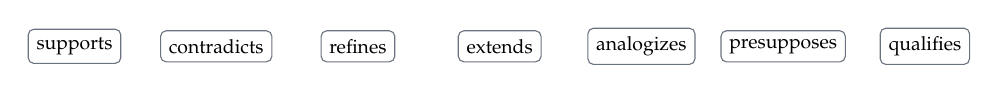
\begin{tikzpicture}[
    rel/.style={draw=midgray, rounded corners=2pt, fill=white, font=\scriptsize, inner sep=3pt},
]
\foreach \name/\x in {supports/0, contradicts/1.8, refines/3.6, extends/5.4, analogizes/7.2, presupposes/9, qualifies/10.8} {
    \node[rel] at (\x, 0) {\name};
}
\end{tikzpicture}
\end{center}

The \texttt{PrincipleDistiller} clusters claims by embedding similarity and synthesises each cluster into a named principle. The \texttt{GraphPersistence} layer handles JSON serialisation.

\subsection{Coherence Engine (\texttt{coherence.py}, ${\sim}900$ lines)}

The heart of Noosphere. Six independently-grounded layers each produce a score in $[0, 1]$:

\begin{center}
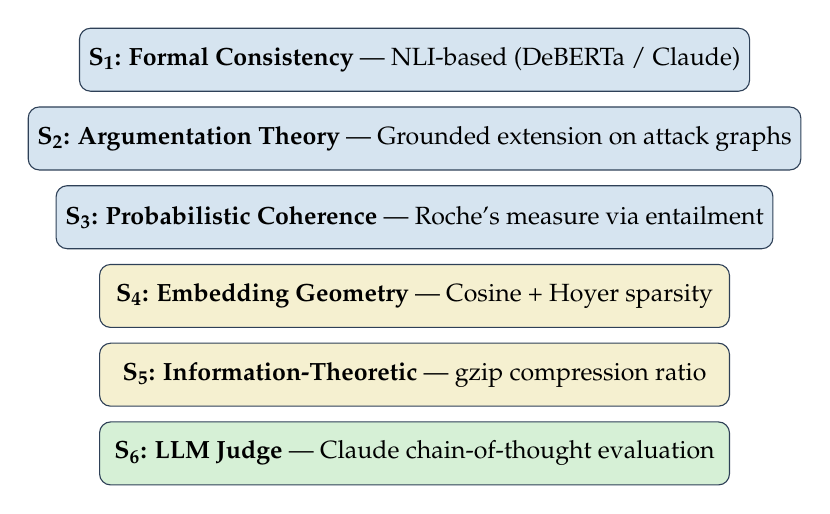
\begin{tikzpicture}[
    layer/.style={draw=accent, rounded corners=4pt, minimum width=8cm, minimum height=0.8cm, align=center, font=\small},
]
\node[layer, fill=softblue] (L1) at (0, 3.0) {\textbf{S\textsubscript{1}: Formal Consistency} --- NLI-based (DeBERTa / Claude)};
\node[layer, fill=softblue] (L2) at (0, 2.0) {\textbf{S\textsubscript{2}: Argumentation Theory} --- Grounded extension on attack graphs};
\node[layer, fill=softblue] (L3) at (0, 1.0) {\textbf{S\textsubscript{3}: Probabilistic Coherence} --- Roche's measure via entailment};
\node[layer, fill=softyellow] (L4) at (0, 0.0) {\textbf{S\textsubscript{4}: Embedding Geometry} --- Cosine + Hoyer sparsity};
\node[layer, fill=softyellow] (L5) at (0,-1.0) {\textbf{S\textsubscript{5}: Information-Theoretic} --- gzip compression ratio};
\node[layer, fill=softgreen] (L6) at (0,-2.0) {\textbf{S\textsubscript{6}: LLM Judge} --- Claude chain-of-thought evaluation};
\end{tikzpicture}
\end{center}

Default weights: $S_1 = 0.25$, $S_2 = 0.10$, $S_3 = 0.15$, $S_4 = 0.15$, $S_5 = 0.10$, $S_6 = 0.25$. The engine also identifies specific contradictions (pairs of principles with high $S_1$ contradiction scores) and weak links (low-coherence edges).

\subsection{Embedding Geometry (\texttt{geometry.py}, ${\sim}400$ lines)}

Implements the \textbf{Embedding Geometry Conjecture}: contradiction between two propositions manifests not as opposite cosine directions but as \emph{concentrated sparsity} in the difference vector $\mathbf{d} = \mathbf{v}_a - \mathbf{v}_b$. Formally, the Hoyer sparsity index
\[
H(\mathbf{d}) = \frac{\sqrt{n} - \|\mathbf{d}\|_1 / \|\mathbf{d}\|_2}{\sqrt{n} - 1}
\]
is significantly higher for contradicting pairs than for merely unrelated pairs. This module also implements the Householder reflection $\mathbf{v}' = \mathbf{v} - 2(\mathbf{v} \cdot \hat{\mathbf{a}})\hat{\mathbf{a}}$ for adversarial argument generation.

\subsection{Temporal Tracker (\texttt{temporal.py}, ${\sim}300$ lines)}

Records \texttt{TemporalSnapshot}s of each principle at every ingestion epoch: conviction level, embedding vector, and drift magnitude from the principle's original embedding. Enables questions like ``How has our thinking on X evolved?'' and ``Which principles have shifted most?''

\subsection{Inference Engine (\texttt{inference.py}, ${\sim}400$ lines)}

Supports four operations: (1) \emph{Principle retrieval} via embedding similarity; (2) \emph{Reasoning chains} that trace entailment paths through the graph; (3) \emph{Adversarial generation} using the Householder reflector; (4) \emph{Consistency checking} that verifies whether a new claim is compatible with the existing graph.

\subsection{Discourse Classifier (\texttt{classifier.py}, ${\sim}200$ lines)}

Classifies each claim into one of five discourse types using Claude with a heuristic fallback:

\begin{center}
\begin{tabular}{ll}
\toprule
\textbf{Type} & \textbf{Description} \\
\midrule
\textsc{Methodological} & How to think, evaluate, or reason \\
\textsc{Substantive} & What is true about the world \\
\textsc{Meta-Methodological} & How to evaluate methods of thinking \\
\textsc{Mixed} & Both methodological and substantive content \\
\textsc{Non-Propositional} & Rhetorical, phatic, or structural utterance \\
\bottomrule
\end{tabular}
\end{center}

This classification drives the routing decision: methodological claims build the ontology graph; substantive claims populate the conclusions registry.

\subsection{Conclusions Registry (\texttt{conclusions.py}, ${\sim}300$ lines)}

A separate store for substantive truth-claims, deliberately isolated from the methodological graph. Each conclusion carries a reasoning method tag, a resolution status (open, confirmed, refuted, superseded), and metadata for calibration tracking.

\subsection{Meta-Analysis (\texttt{meta\_analysis.py}, ${\sim}200$ lines)}

Extracts methodological observations from discourse: instances where speakers reflect on their own reasoning, identify biases, or characterise their epistemic approach.

\subsection{Founder Registry (\texttt{founders.py}, ${\sim}200$ lines)}

Maintains persistent founder profiles with intellectual fingerprints. Every claim is attributed to a founder; every principle carries weighted contribution records showing each founder's intellectual influence on the collective body of thought.

\subsection{Synthesis Engine (\texttt{synthesis.py}, ${\sim}500$ lines)}
\label{sec:synthesis}

Runs automatically after every ingestion. Produces five outputs:

\begin{enumerate}
\item \textbf{Discussion Summary} --- Structured LLM-generated summary of the episode.
\item \textbf{Manuscript Update} --- Extends a running book manuscript (\texttt{synthesis/manuscript.md}) that grows with every discussion, accumulating and refining the firm's thought.
\item \textbf{Next Questions} --- Questions generated from: contradictions detected via Hoyer sparsity, underexplored principles, and themes from the latest discussion.
\item \textbf{Source Recommendations} --- Embedding-space cosine similarity matching against a curated catalogue of 16+ sources. Includes contradiction-targeted matching: sources are recommended for the \emph{midpoints} of contradicting principle pairs.
\item \textbf{Contradiction Report} --- Full Hoyer-sparsity-based contradiction analysis with LLM-generated resolution strategies.
\end{enumerate}

\subsection{CLI (\texttt{cli.py}, ${\sim}400$ lines)}

Click-based command-line interface exposing all major operations: \texttt{ingest}, \texttt{ask}, \texttt{graph}, \texttt{coherence}, \texttt{evolution}, \texttt{stats}, \texttt{search}, \texttt{synthesis}.

% ====================================================================
\section{Founder Portal}

\subsection{Architecture}

The Founder Portal is a Next.js 16 application (React 19, TypeScript) that provides an authenticated web interface for founders. It communicates with Noosphere Core via subprocess invocation.

\begin{center}
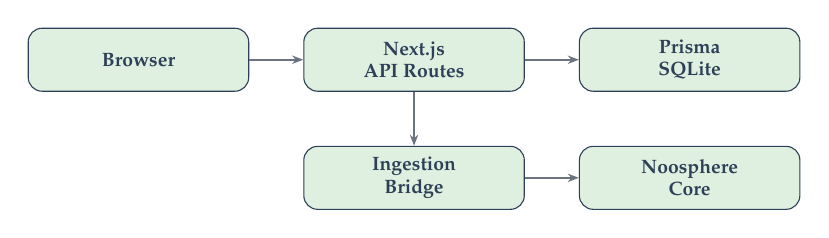
\begin{tikzpicture}[
    box/.style={draw=accent, rounded corners=5pt, minimum width=2.8cm, minimum height=0.8cm, align=center, font=\scriptsize\bfseries, fill=portalbg, text=accent},
    arrow/.style={-{Stealth[length=4pt]}, thick, color=midgray},
]
\node[box] (browser) at (0,0) {Browser};
\node[box] (nextjs) at (3.5,0) {Next.js\\API Routes};
\node[box] (prisma) at (7,0) {Prisma\\SQLite};
\node[box] (ingest) at (3.5,-1.5) {Ingestion\\Bridge};
\node[box] (noo) at (7,-1.5) {Noosphere\\Core};

\draw[arrow] (browser) -- (nextjs);
\draw[arrow] (nextjs) -- (prisma);
\draw[arrow] (nextjs) -- (ingest);
\draw[arrow] (ingest) -- (noo);
\end{tikzpicture}
\end{center}

\subsection{Database Schema}

Four tables via Prisma: \textbf{Founder} (id, name, email, role, \texttt{noosphereId}), \textbf{Session} (token-based auth, 30-day expiry), \textbf{Upload} (file metadata, processing status, claim counts), \textbf{AuditEvent} (action log).

\subsection{Ingestion Pipeline}

When a founder uploads a file (essay, PDF, audio), the portal:

\begin{enumerate}
\item Saves the file to disk and creates an \texttt{Upload} record (status: \texttt{pending}).
\item Asynchronously triggers the ingestion bridge, which:
\begin{itemize}
\item Extracts text (via \texttt{pdftotext}, \texttt{pandoc}, or direct read).
\item Transcribes audio (via OpenAI Whisper API) if applicable.
\item Spawns a Python subprocess calling \texttt{NoosphereOrchestrator.ingest\_written\_input()}.
\end{itemize}
\item Updates the \texttt{Upload} record with claim counts and status (\texttt{ingested} or \texttt{failed}).
\item Logs an \texttt{AuditEvent}.
\end{enumerate}

\subsection{Pages}

The portal exposes: a landing page, login, a founder dashboard (upload history, claim/principle counts, status badges), a file upload form, and a founder discovery page.

% ====================================================================
\section{Dialectic: Live Conversation Analysis}

Dialectic is the newest subsystem---a macOS desktop application that provides \textbf{real-time epistemological feedback} during live discussions. It is the live, in-conversation counterpart to Noosphere's post-hoc analysis.

\subsection{Motivation}

Noosphere analyses discussions after they happen. But many of the most important interventions---noticing a contradiction as it forms, flagging an open loop before it's forgotten, suggesting a question that would deepen the current thread---require \emph{real-time} analysis. Dialectic fills this gap.

\subsection{Architecture}

Dialectic comprises four modules feeding a PyQt6 dashboard:

\subsubsection{Audio Engine (\texttt{audio.py})}
Captures audio from the system microphone (or a BlackHole aggregate device for system audio routing) via \texttt{sounddevice}. Records at 16\,kHz/16-bit mono. Simultaneously archives to WAV and feeds chunks to the transcriber. Latency: ${\sim}64$\,ms per buffer at 1024 samples.

\subsubsection{Transcriber (\texttt{transcriber.py})}
Converts audio to text in near-real-time using \texttt{faster-whisper} (CTranslate2 backend, INT8 quantisation). Accumulates audio until a natural silence break or maximum duration (${\sim}8$\,s), then transcribes the chunk. Can be swapped for a cloud backend (AssemblyAI) for lower latency and speaker diarisation.

Latency budget: ${\sim}2{-}3$\,s per chunk with local Whisper; ${\sim}300$\,ms with AssemblyAI streaming.

\subsubsection{Live Analyzer (\texttt{analyzer.py})}
Runs four parallel analysis pipelines on each new transcript segment:

\textbf{1. Contradiction Detection.} A DeBERTa-v3-small cross-encoder (\texttt{cross-encoder/nli-deberta-v3-small}) checks each new utterance against the last 8 statements in a sliding window. Pairs exceeding a contradiction score of 0.6 are flagged. Latency: ${\sim}60$\,ms per check.

\textbf{2. Topic Tracking.} Each sentence is embedded with MiniLM-L6-v2 (${\sim}40$\,ms). Every 4 sentences, the sliding window (40 sentences) is re-clustered using DBSCAN with cosine distance. The dominant cluster defines the ``current topic''; utterances in other clusters signal drift. Keywords are extracted via term frequency.

\textbf{3. Open-Loop Detection.} Questions and deferral language (``let's come back to that'', ``park that for now'') open loops. Each loop is tracked by embedding similarity to subsequent utterances. If a loop is not referenced within 2 minutes, it is flagged as \textbf{abandoned}---the conversation has moved on without closing it.

\textbf{4. Question Generation.} Every 45 seconds, a prompt is sent to Claude (or a local LLM via Ollama) with the recent transcript, open loops, and current topic. The prompt prioritises: probing unexamined assumptions, addressing abandoned loops, sharpening contradictions, and pushing toward falsifiable claims.

\subsubsection{Dashboard (\texttt{dashboard.py})}

A PyQt6 application with five live-updating panels:

\begin{center}
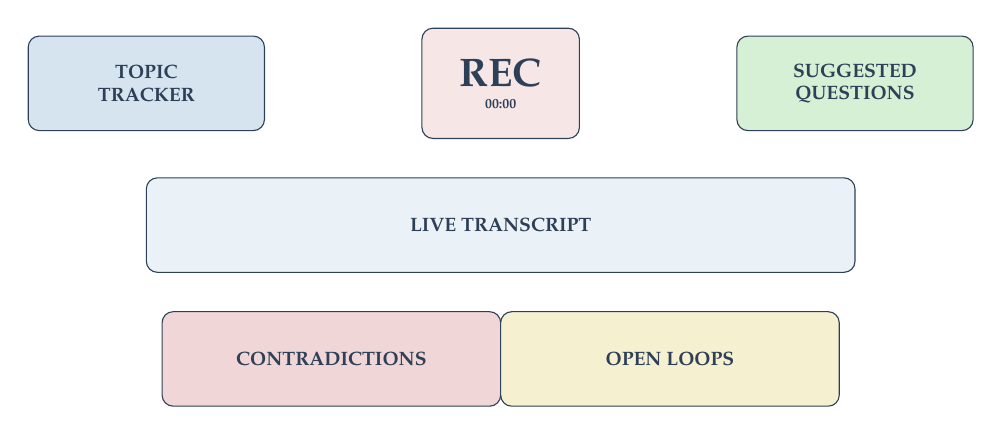
\begin{tikzpicture}[
    panel/.style={draw=accent, rounded corners=4pt, minimum height=1.2cm, align=center, font=\scriptsize\bfseries, text=accent},
]
\node[panel, fill=softblue, minimum width=3cm] (topics) at (0, 1.5) {TOPIC\\TRACKER};
\node[panel, fill=softred!60, minimum width=2cm, minimum height=1.4cm] (rec) at (4.5, 1.5) {\Large REC\\{\tiny 00:00}};
\node[panel, fill=softgreen, minimum width=3cm] (qs) at (9, 1.5) {SUGGESTED\\QUESTIONS};
\node[panel, fill=softblue!50, minimum width=9cm] (transcript) at (4.5, -0.3) {LIVE TRANSCRIPT};
\node[panel, fill=softred, minimum width=4.3cm] (contra) at (2.35, -2) {CONTRADICTIONS};
\node[panel, fill=softyellow, minimum width=4.3cm] (loops) at (6.65, -2) {OPEN LOOPS};
\end{tikzpicture}
\end{center}

The record button is centred at the top with a running timer. The transcript scrolls below it. Analysis feeds flank the sides and bottom, updating in real time as the recording continues.

\subsection{Latency Budget}

\begin{center}
\begin{tabular}{lr}
\toprule
\textbf{Stage} & \textbf{Latency} \\
\midrule
Audio capture (buffer fill) & ${\sim}64$\,ms \\
Transcription (local Whisper) & ${\sim}2{-}3$\,s \\
Transcription (AssemblyAI cloud) & ${\sim}300$\,ms \\
NLI contradiction check & ${\sim}60$\,ms \\
Embedding + topic cluster & ${\sim}50$\,ms \\
Question generation (Claude) & ${\sim}500$\,ms \\
UI render & $<16$\,ms \\
\midrule
\textbf{Total (cloud path)} & ${\sim}500$\,ms \\
\textbf{Total (local path)} & ${\sim}3$\,s \\
\bottomrule
\end{tabular}
\end{center}

\subsection{Future Integration}

Dialectic currently operates independently. The planned integration path:

\begin{itemize}
\item \textbf{Live-to-Noosphere bridge}: At the end of a recording session, the full transcript and all detected claims are dispatched to Noosphere's ingestion pipeline for permanent incorporation into the knowledge graph.
\item \textbf{Real-time graph queries}: During a conversation, Dialectic will query Noosphere for existing principles related to the current topic, surfacing relevant prior commitments and potential conflicts with already-held positions.
\item \textbf{Speaker diarisation}: Integration with AssemblyAI's real-time speaker identification or pyannote for automatic founder attribution during live recording.
\end{itemize}

% ====================================================================
\section{Research Infrastructure}

\subsection{Embedding Geometry Conjecture}

The \texttt{ideologicalOntology/} directory contains the original experimental validation of the Embedding Geometry Conjecture, including:

\begin{itemize}
\item \texttt{simulation\_synthetic.py} --- Synthetic contradiction generation and Hoyer-sparsity measurement.
\item \texttt{experiment\_real\_models.py} --- Validation on real sentence embeddings.
\item \texttt{experiment\_contradiction\_direction.py} --- PCA-based contradiction direction learning.
\item \texttt{contradiction\_detector.py} --- Ontological mapping and geometry-based contradiction detection.
\end{itemize}

\subsection{Research Documents}

The \texttt{docs/} folder contains LaTeX-compiled research documents:

\begin{tabularx}{\textwidth}{lX}
\toprule
\textbf{Document} & \textbf{Content} \\
\midrule
Server Architecture & System topology, component architecture, data flow, deployment strategy \\
Founders Questions & 12 philosophical questions for podcast discussions \\
Transcript Extraction Research & 7 NLP approaches for extracting settled positions from transcripts \\
Podcast Infrastructure Research & End-to-end podcast automation pipeline design \\
Geometry of Unresolution & 12 mathematical frameworks for modelling incomplete epistemic states \\
\bottomrule
\end{tabularx}

% ====================================================================
\section{Dependency Stack}

\subsection{Noosphere Core}

\begin{center}
\begin{tabular}{lll}
\toprule
\textbf{Package} & \textbf{Version} & \textbf{Role} \\
\midrule
\texttt{sentence-transformers} & $\geq 2.2$ & SBERT embeddings (MiniLM-L6-v2) \\
\texttt{numpy} & $\geq 1.24$ & Linear algebra \\
\texttt{scipy} & $\geq 1.10$ & Signal processing, spatial distance \\
\texttt{scikit-learn} & $\geq 1.2$ & Clustering, PCA, metrics \\
\texttt{networkx} & $\geq 3.0$ & Knowledge graph \\
\texttt{anthropic} & $\geq 0.39$ & Claude API \\
\texttt{spacy} & $\geq 3.5$ & NLP pipeline \\
\texttt{pydantic} & $\geq 2.0$ & Data validation \\
\texttt{click} & $\geq 8.1$ & CLI framework \\
\texttt{rich} & $\geq 13.0$ & Terminal formatting \\
\bottomrule
\end{tabular}
\end{center}

\subsection{Founder Portal}

Next.js 16, React 19, TypeScript, Prisma 7, SQLite, bcryptjs, Tailwind CSS 4.

\subsection{Dialectic}

\begin{center}
\begin{tabular}{lll}
\toprule
\textbf{Package} & \textbf{Version} & \textbf{Role} \\
\midrule
\texttt{PyQt6} & $\geq 6.6$ & Dashboard GUI \\
\texttt{sounddevice} & $\geq 0.4.6$ & Audio capture \\
\texttt{faster-whisper} & $\geq 1.0$ & Local transcription \\
\texttt{sentence-transformers} & $\geq 2.6$ & Embeddings + NLI \\
\texttt{scikit-learn} & $\geq 1.2$ & DBSCAN topic clustering \\
\texttt{anthropic} & $\geq 0.39$ & Claude API for questions \\
\bottomrule
\end{tabular}
\end{center}

% ====================================================================
\section{Project Status and Roadmap}

\subsection{Current State}

\begin{center}
\begin{tabular}{lcl}
\toprule
\textbf{Component} & \textbf{Status} & \textbf{Notes} \\
\midrule
Noosphere Core (all 15 modules) & \color{teal}\textbf{Complete} & All modules pass AST validation \\
Coherence Engine (6 layers) & \color{teal}\textbf{Complete} & Weights configurable \\
Embedding Geometry & \color{teal}\textbf{Complete} & Hoyer sparsity + Householder reflection \\
Synthesis Engine & \color{teal}\textbf{Complete} & 5 output types operational \\
CLI & \color{teal}\textbf{Complete} & All commands wired \\
Founder Portal (auth, upload, dashboard) & \color{teal}\textbf{Complete} & Seed script, ingestion bridge \\
Dialectic (v0.1 framework) & \color{amber}\textbf{Alpha} & UI + pipeline architecture built \\
Speaker diarisation & \color{deepred}\textbf{Planned} & Requires AssemblyAI or pyannote \\
Dialectic $\leftrightarrow$ Noosphere bridge & \color{deepred}\textbf{Planned} & Post-session ingestion \\
Persistent homology diagnostics & \color{deepred}\textbf{Planned} & Research complete, implementation pending \\
Sheaf cohomology checks & \color{deepred}\textbf{Planned} & Research complete, implementation pending \\
\bottomrule
\end{tabular}
\end{center}

\subsection{Immediate Next Steps}

\begin{enumerate}
\item \textbf{Dialectic hardening}: Install dependencies on the local Mac, test audio capture, tune transcription latency, validate NLI model inference speed.
\item \textbf{AssemblyAI integration}: Replace local Whisper with AssemblyAI streaming for sub-second transcription with speaker diarisation.
\item \textbf{Live-to-Noosphere bridge}: At session end, dispatch the full transcript through the standard ingestion pipeline.
\item \textbf{Persistent homology module}: Implement Vietoris--Rips filtration on the claim embedding space, compute persistence diagrams, and surface long-lived $H_1$ classes as dialectical loops.
\item \textbf{End-to-end test}: Ingest a real podcast episode through the full pipeline (recording $\to$ transcription $\to$ Noosphere ingestion $\to$ synthesis outputs) and validate all outputs.
\end{enumerate}

\subsection{Long-Term Vision}

The long-term target is a closed loop: Dialectic captures the live discussion, Noosphere analyses it in depth after the fact, the synthesis engine generates the next set of questions, and those questions feed back into the next discussion---a self-improving epistemological cycle with the geometry of unresolution as its diagnostic instrument and the five meta-methodological criteria (progressivity, severity, coherence, compressibility, domain sensitivity) as its evaluative standard.

\vspace{1cm}
\begin{center}
\rule{3cm}{0.4pt}
\end{center}

\end{document}
